\documentclass[tikz,border=5pt]{standalone}
\usepackage{tikz}
\usetikzlibrary{arrows.meta,positioning}
\begin{document}
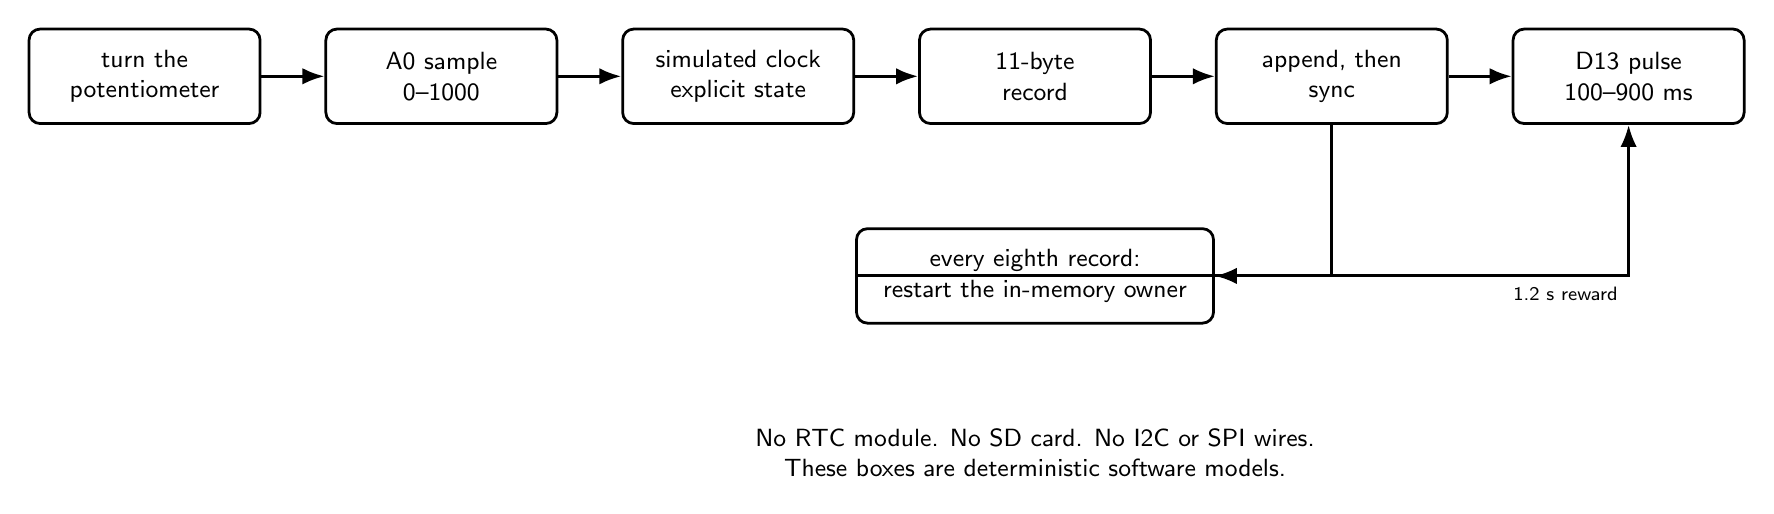
\begin{tikzpicture}[>=Latex,node distance=8mm,
  box/.style={draw,line width=1pt,rounded corners,minimum height=12mm,
    text width=27mm,align=center,font=\sffamily\small},
  arrow/.style={->,line width=1.1pt}]
  \node[box] (turn) {turn the\\potentiometer};
  \node[box,right=of turn] (sample) {A0 sample\\0--1000};
  \node[box,right=of sample] (clock) {simulated clock\\explicit state};
  \node[box,right=of clock] (record) {11-byte\\record};
  \node[box,right=of record] (sync) {append, then\\sync};
  \node[box,right=of sync] (light) {D13 pulse\\100--900 ms};
  \draw[arrow] (turn)--(sample);
  \draw[arrow] (sample)--(clock);
  \draw[arrow] (clock)--(record);
  \draw[arrow] (record)--(sync);
  \draw[arrow] (sync)--(light);
  \node[box,below=13mm of record,text width=43mm] (restart)
    {every eighth record:\\restart the in-memory owner};
  \draw[arrow] (sync.south) |- (restart.east);
  \draw[arrow] (restart.west) -| node[below left,font=\sffamily\scriptsize]
    {1.2 s reward} (light.south);
  \node[font=\sffamily\small,align=center,below=12mm of restart]
    {No RTC module. No SD card. No I2C or SPI wires.\\
     These boxes are deterministic software models.};
\end{tikzpicture}
\end{document}
